%----TEMPLATE FOR Standalone for k
\documentclass[12pt]{article}
\usepackage{geometry}
\usepackage{amssymb} \usepackage{graphicx}  
\usepackage[parfill]{parskip}
\usepackage{graphicx}
\usepackage[table]{xcolor}
\usepackage{rotating}
\usepackage{color}
\usepackage{tikz}
\usetikzlibrary{positioning}
\usepackage{sectsty}
\usepackage{xcolor}% http://ctan.org/pkg/xcolor
\sectionfont{\color{red}}
\subsectionfont{\color{green!80!black}}
\subsubsectionfont{\color{blue!50!white}}
\setlength{\parindent}{.75cm} %%%%%%%  PAGE LAYOUT STUFF
\setlength{\topmargin}{0.25in}
\setlength{\textwidth}{120mm}
\setlength{\textheight}{190mm} % was 9
\setlength{\oddsidemargin}{0.05in}
\setlength{\evensidemargin}{\oddsidemargin}
\headsep=4ex
\parsep=0pt
\parskip=0pt
\newsavebox\FrameBox \newenvironment{Frame}{\vspace{20pt}  \par\setbox\FrameBox\hbox\bgroup\minipage{0.9\textwidth}\parskip\baselineskip\ignorespaces}
	{  \endminipage\egroup\fbox{\box\FrameBox}\par
	\vspace{20pt}}
\title{notes from Whiteboard session}
\author{David, Kirsten}
\begin{document}
\section{Missing from the current model}

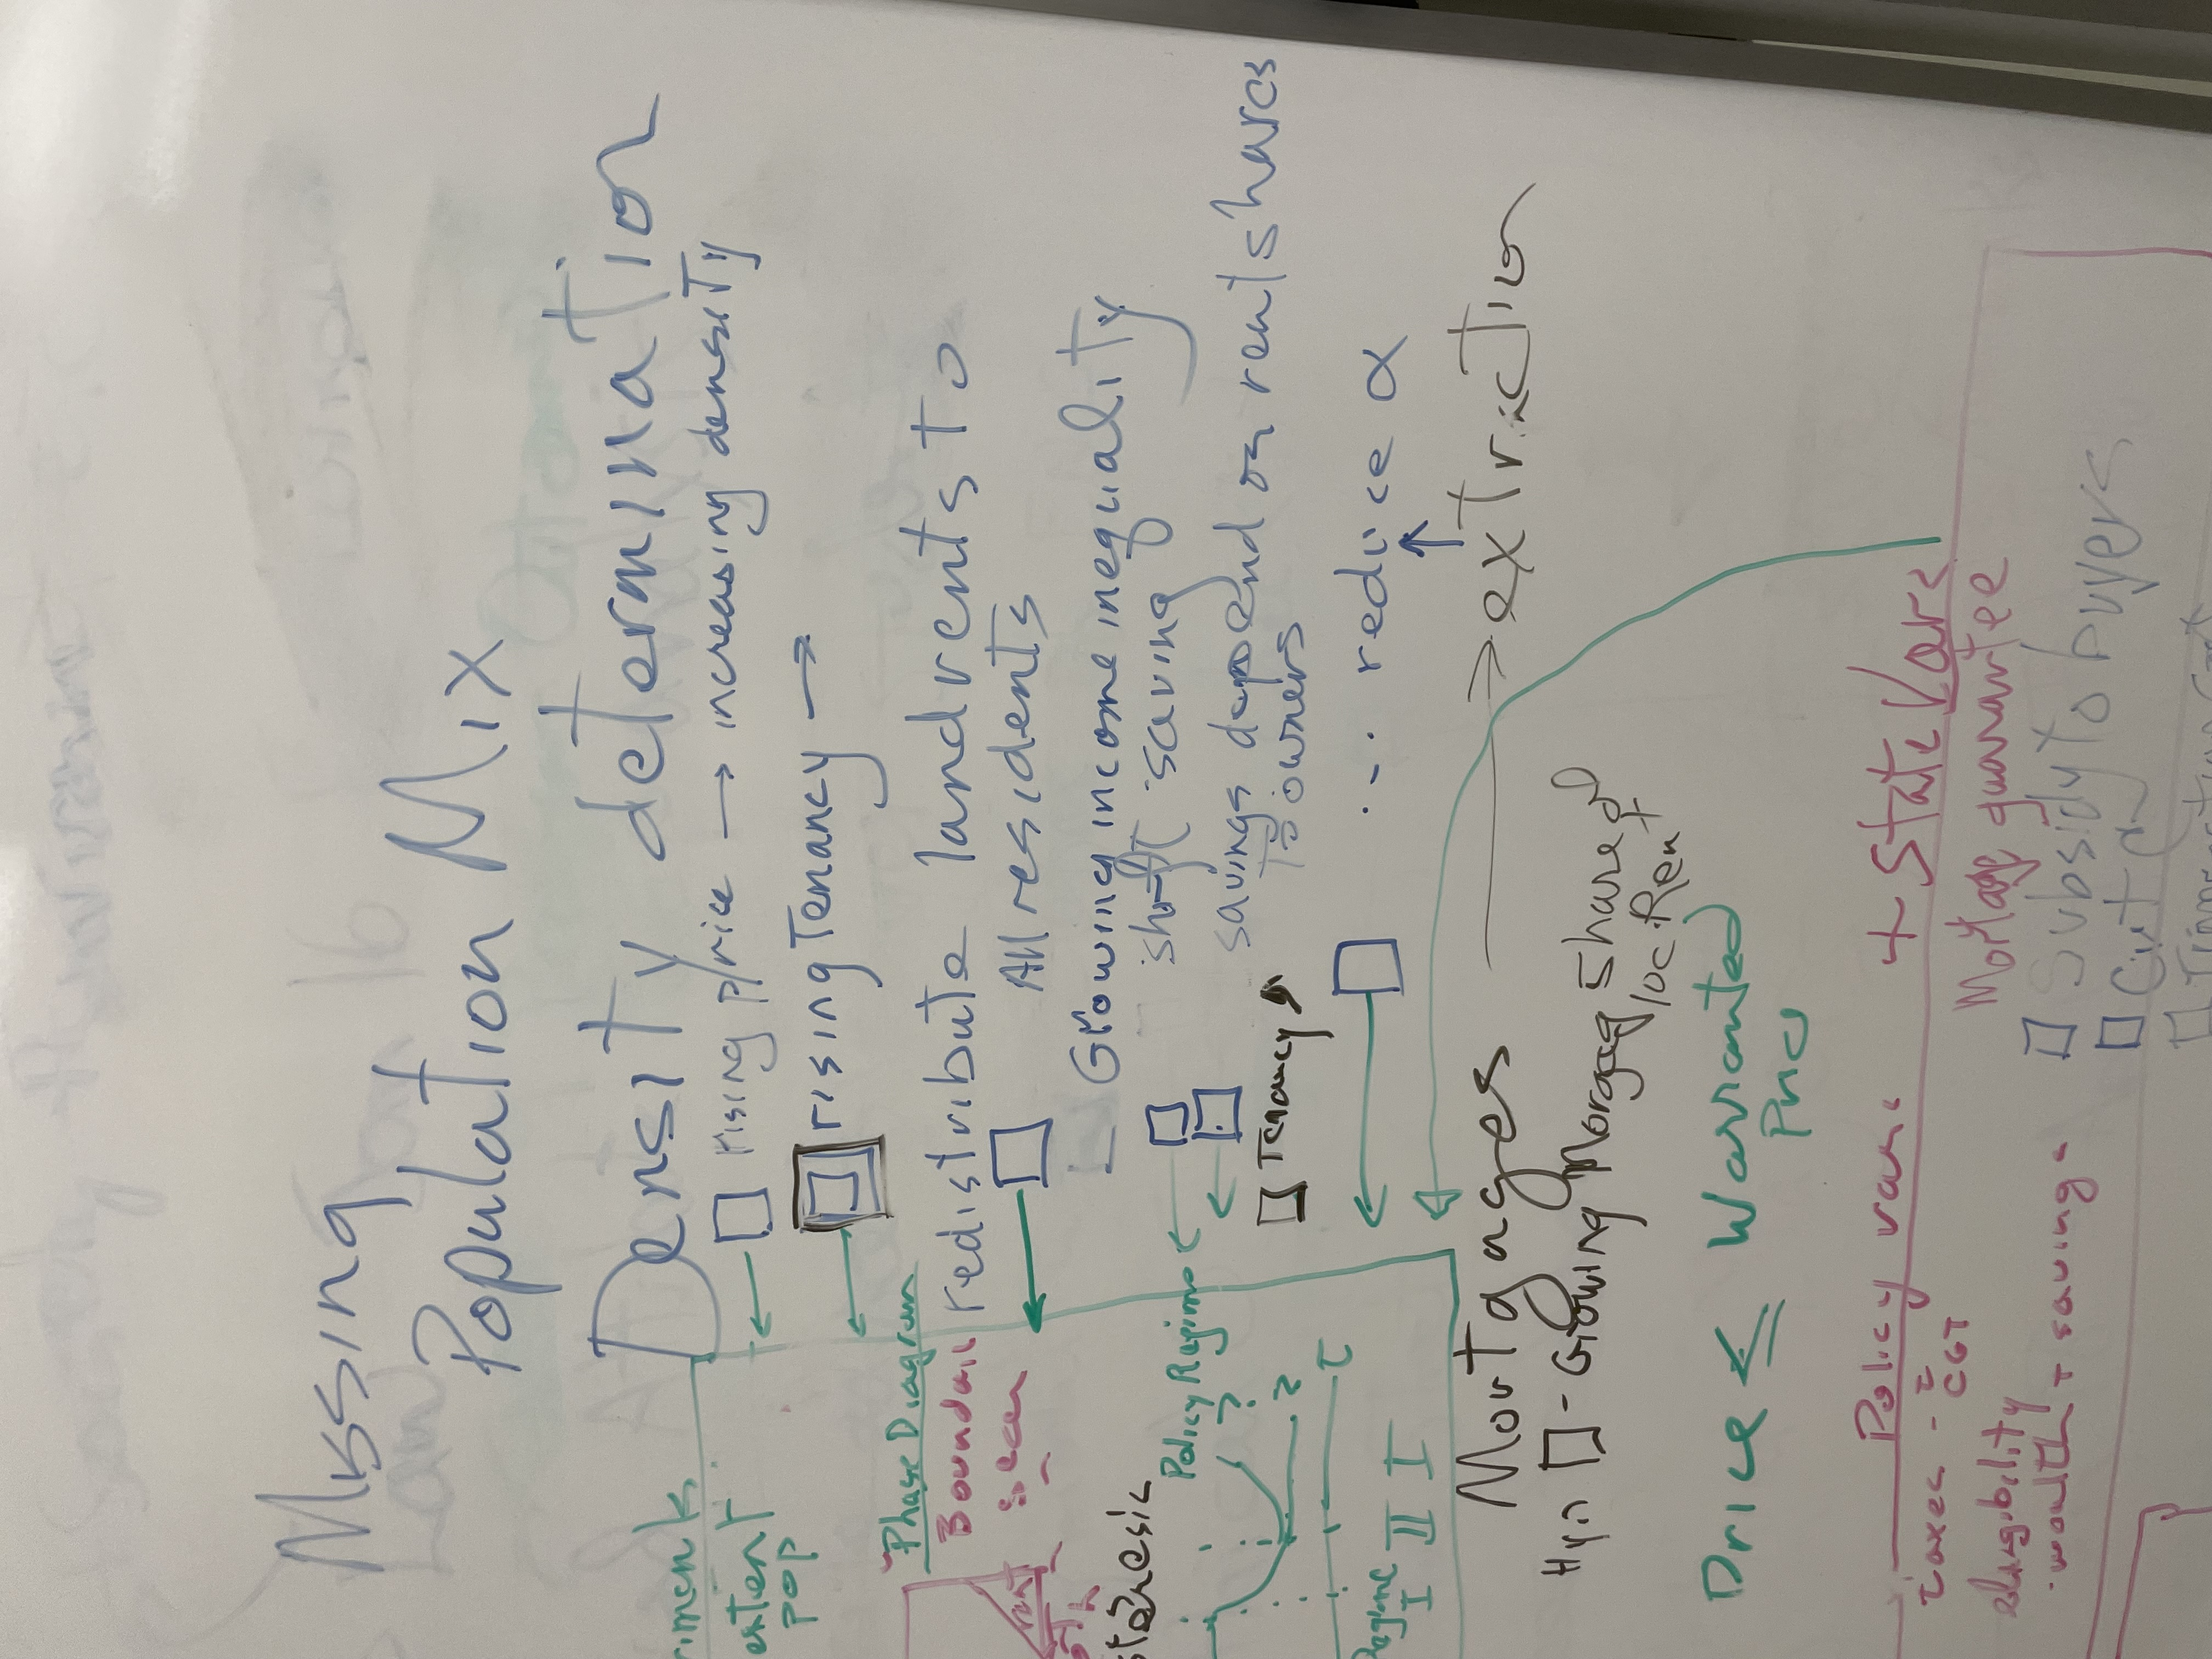
\includegraphics[scale=.4, angle=-90]{IMG_2688.jpg}

\begin{enumerate}
\item  Density determination
   \begin{enumerate}
         \item  Link rising land price to density
         \item  Link rising land tenancy price to density
    \end{enumerate}   
\item explicit distribution of land rent
     \begin{enumerate}
         \item  collect rent and use it for augmenting productivity
         \item redistribute land rents to all residents
         \item apply land rents to amenity for residents
     \end{enumerate}
    
    \item Growing income inequality
     \begin{enumerate}
         \item  Savings rate could depend on rent share for owners
         \item possibly shift the savings function (what was this?)
    \end{enumerate}
    
    \item 
    \begin{enumerate}
         \item  mm
    \end{enumerate}
\end{enumerate}

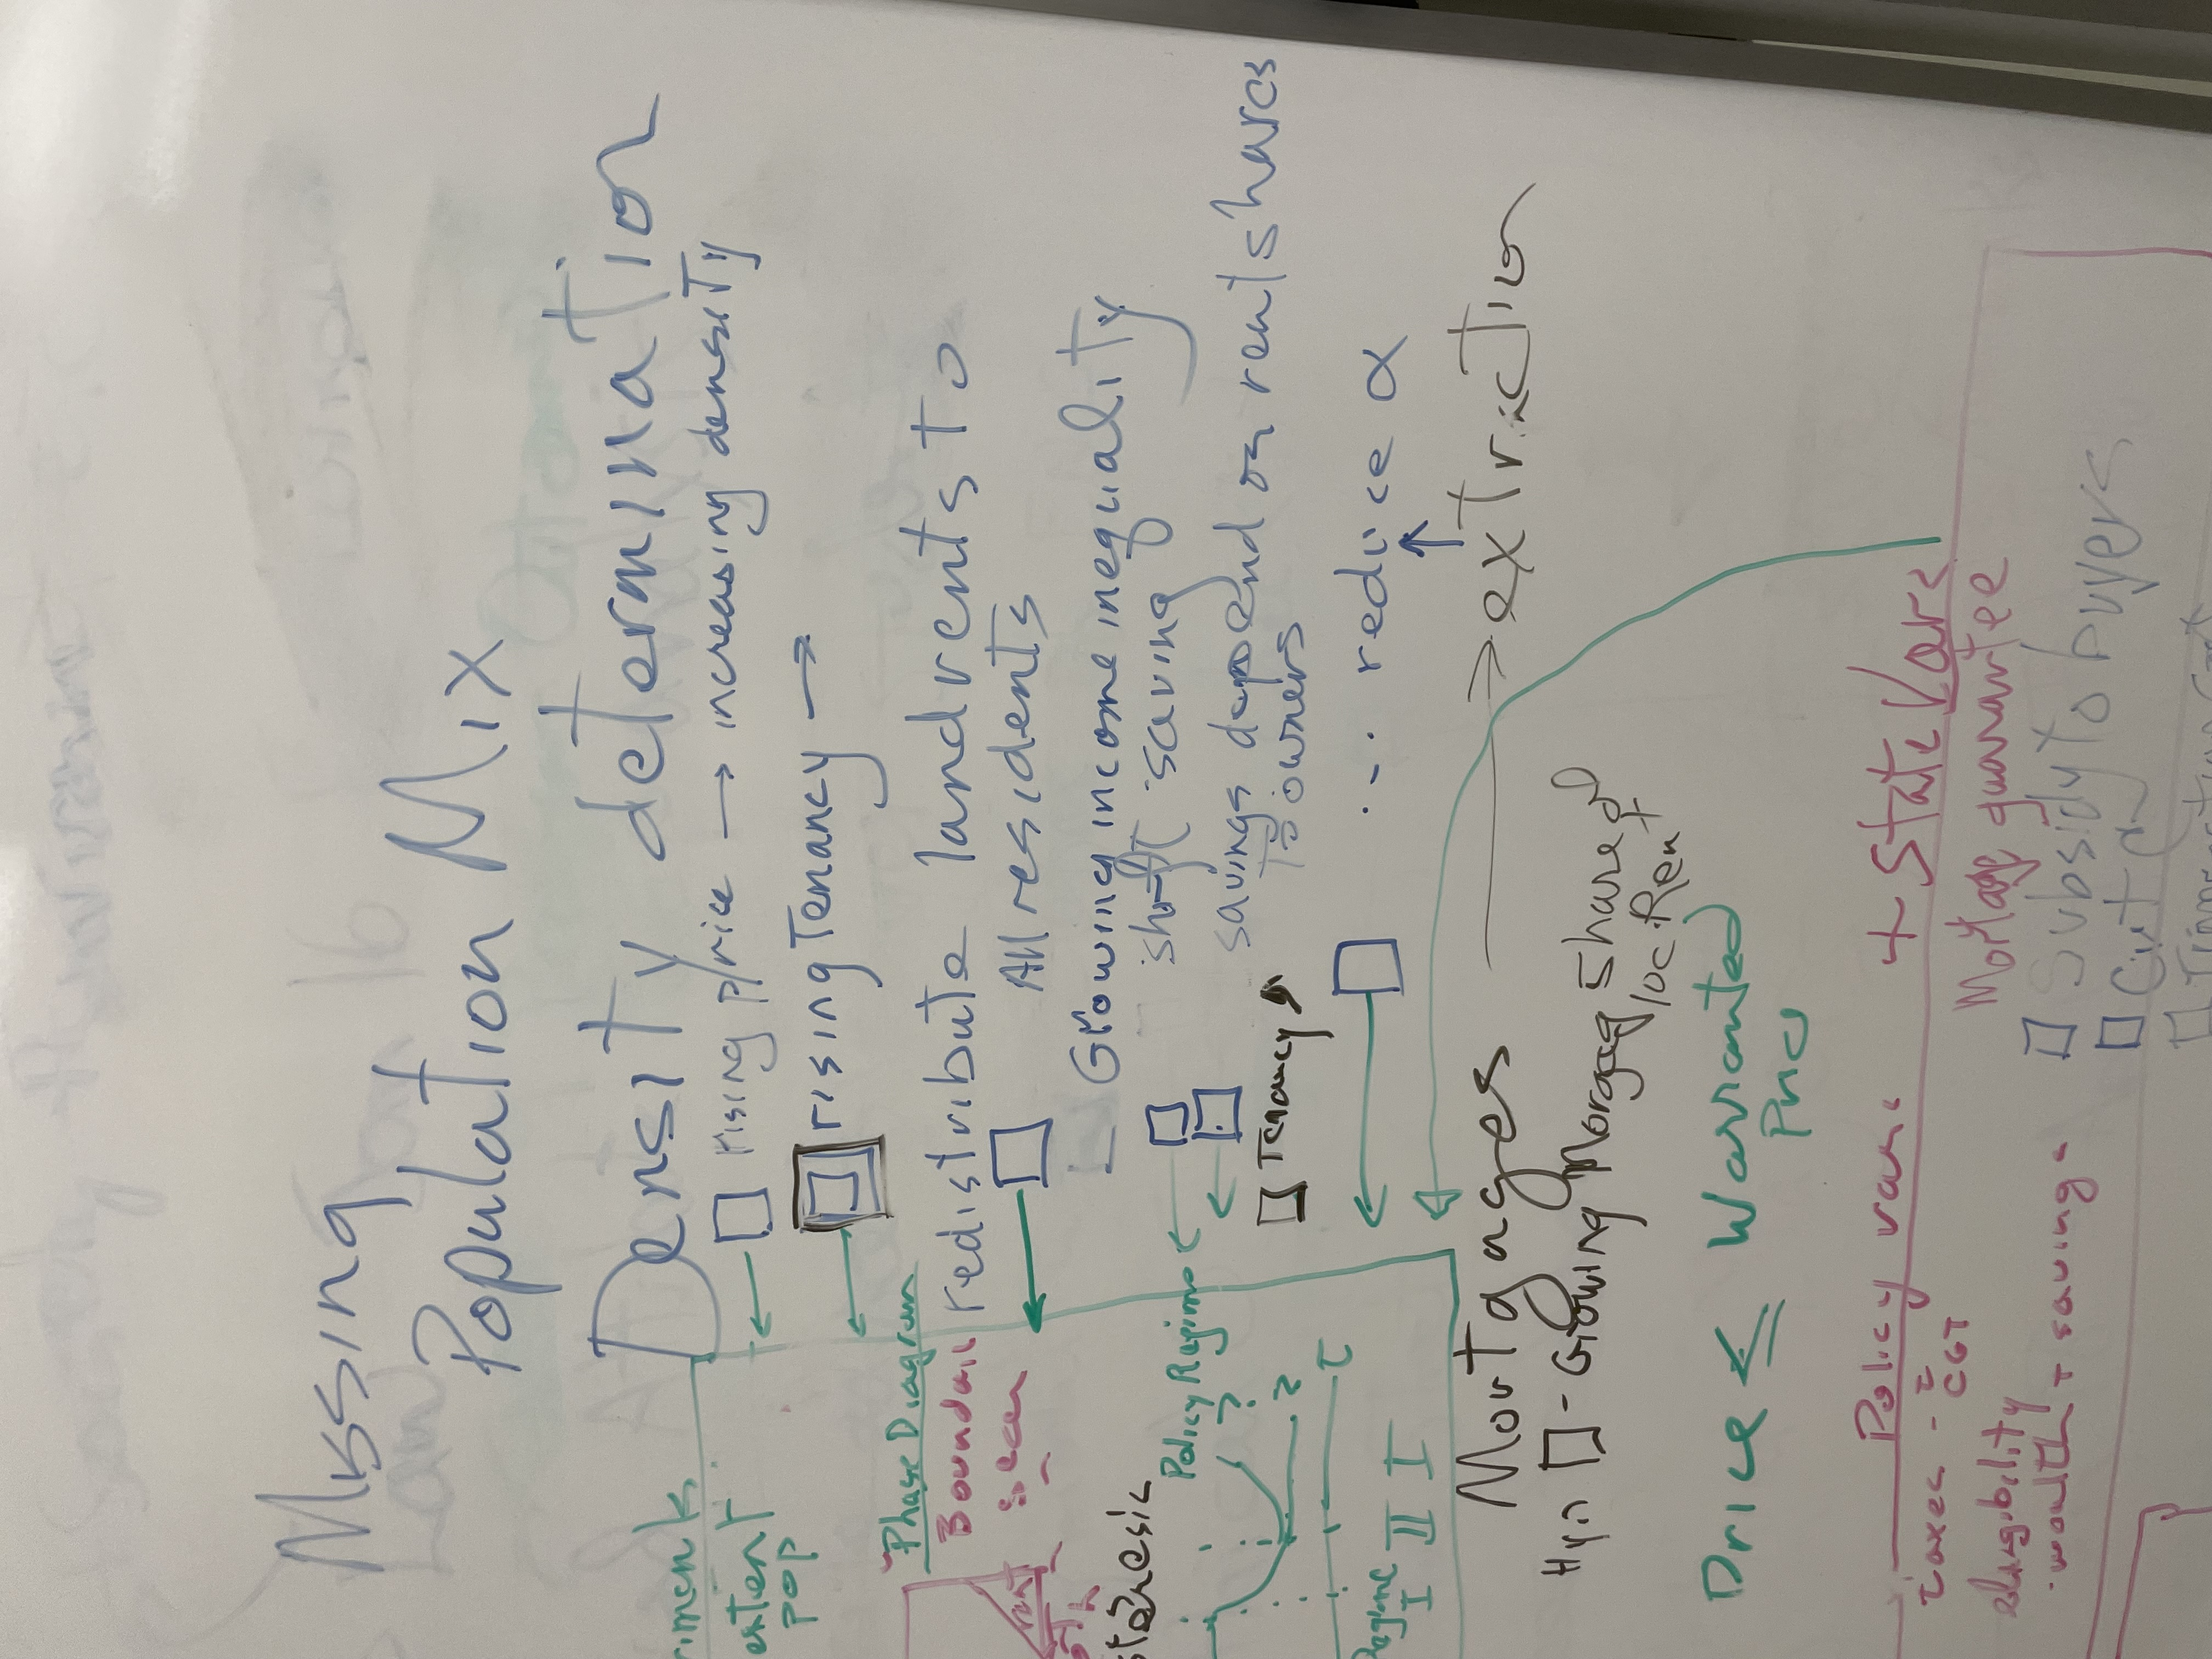
\includegraphics[scale=.5, angle=-90]{IMG_2688.jpg}

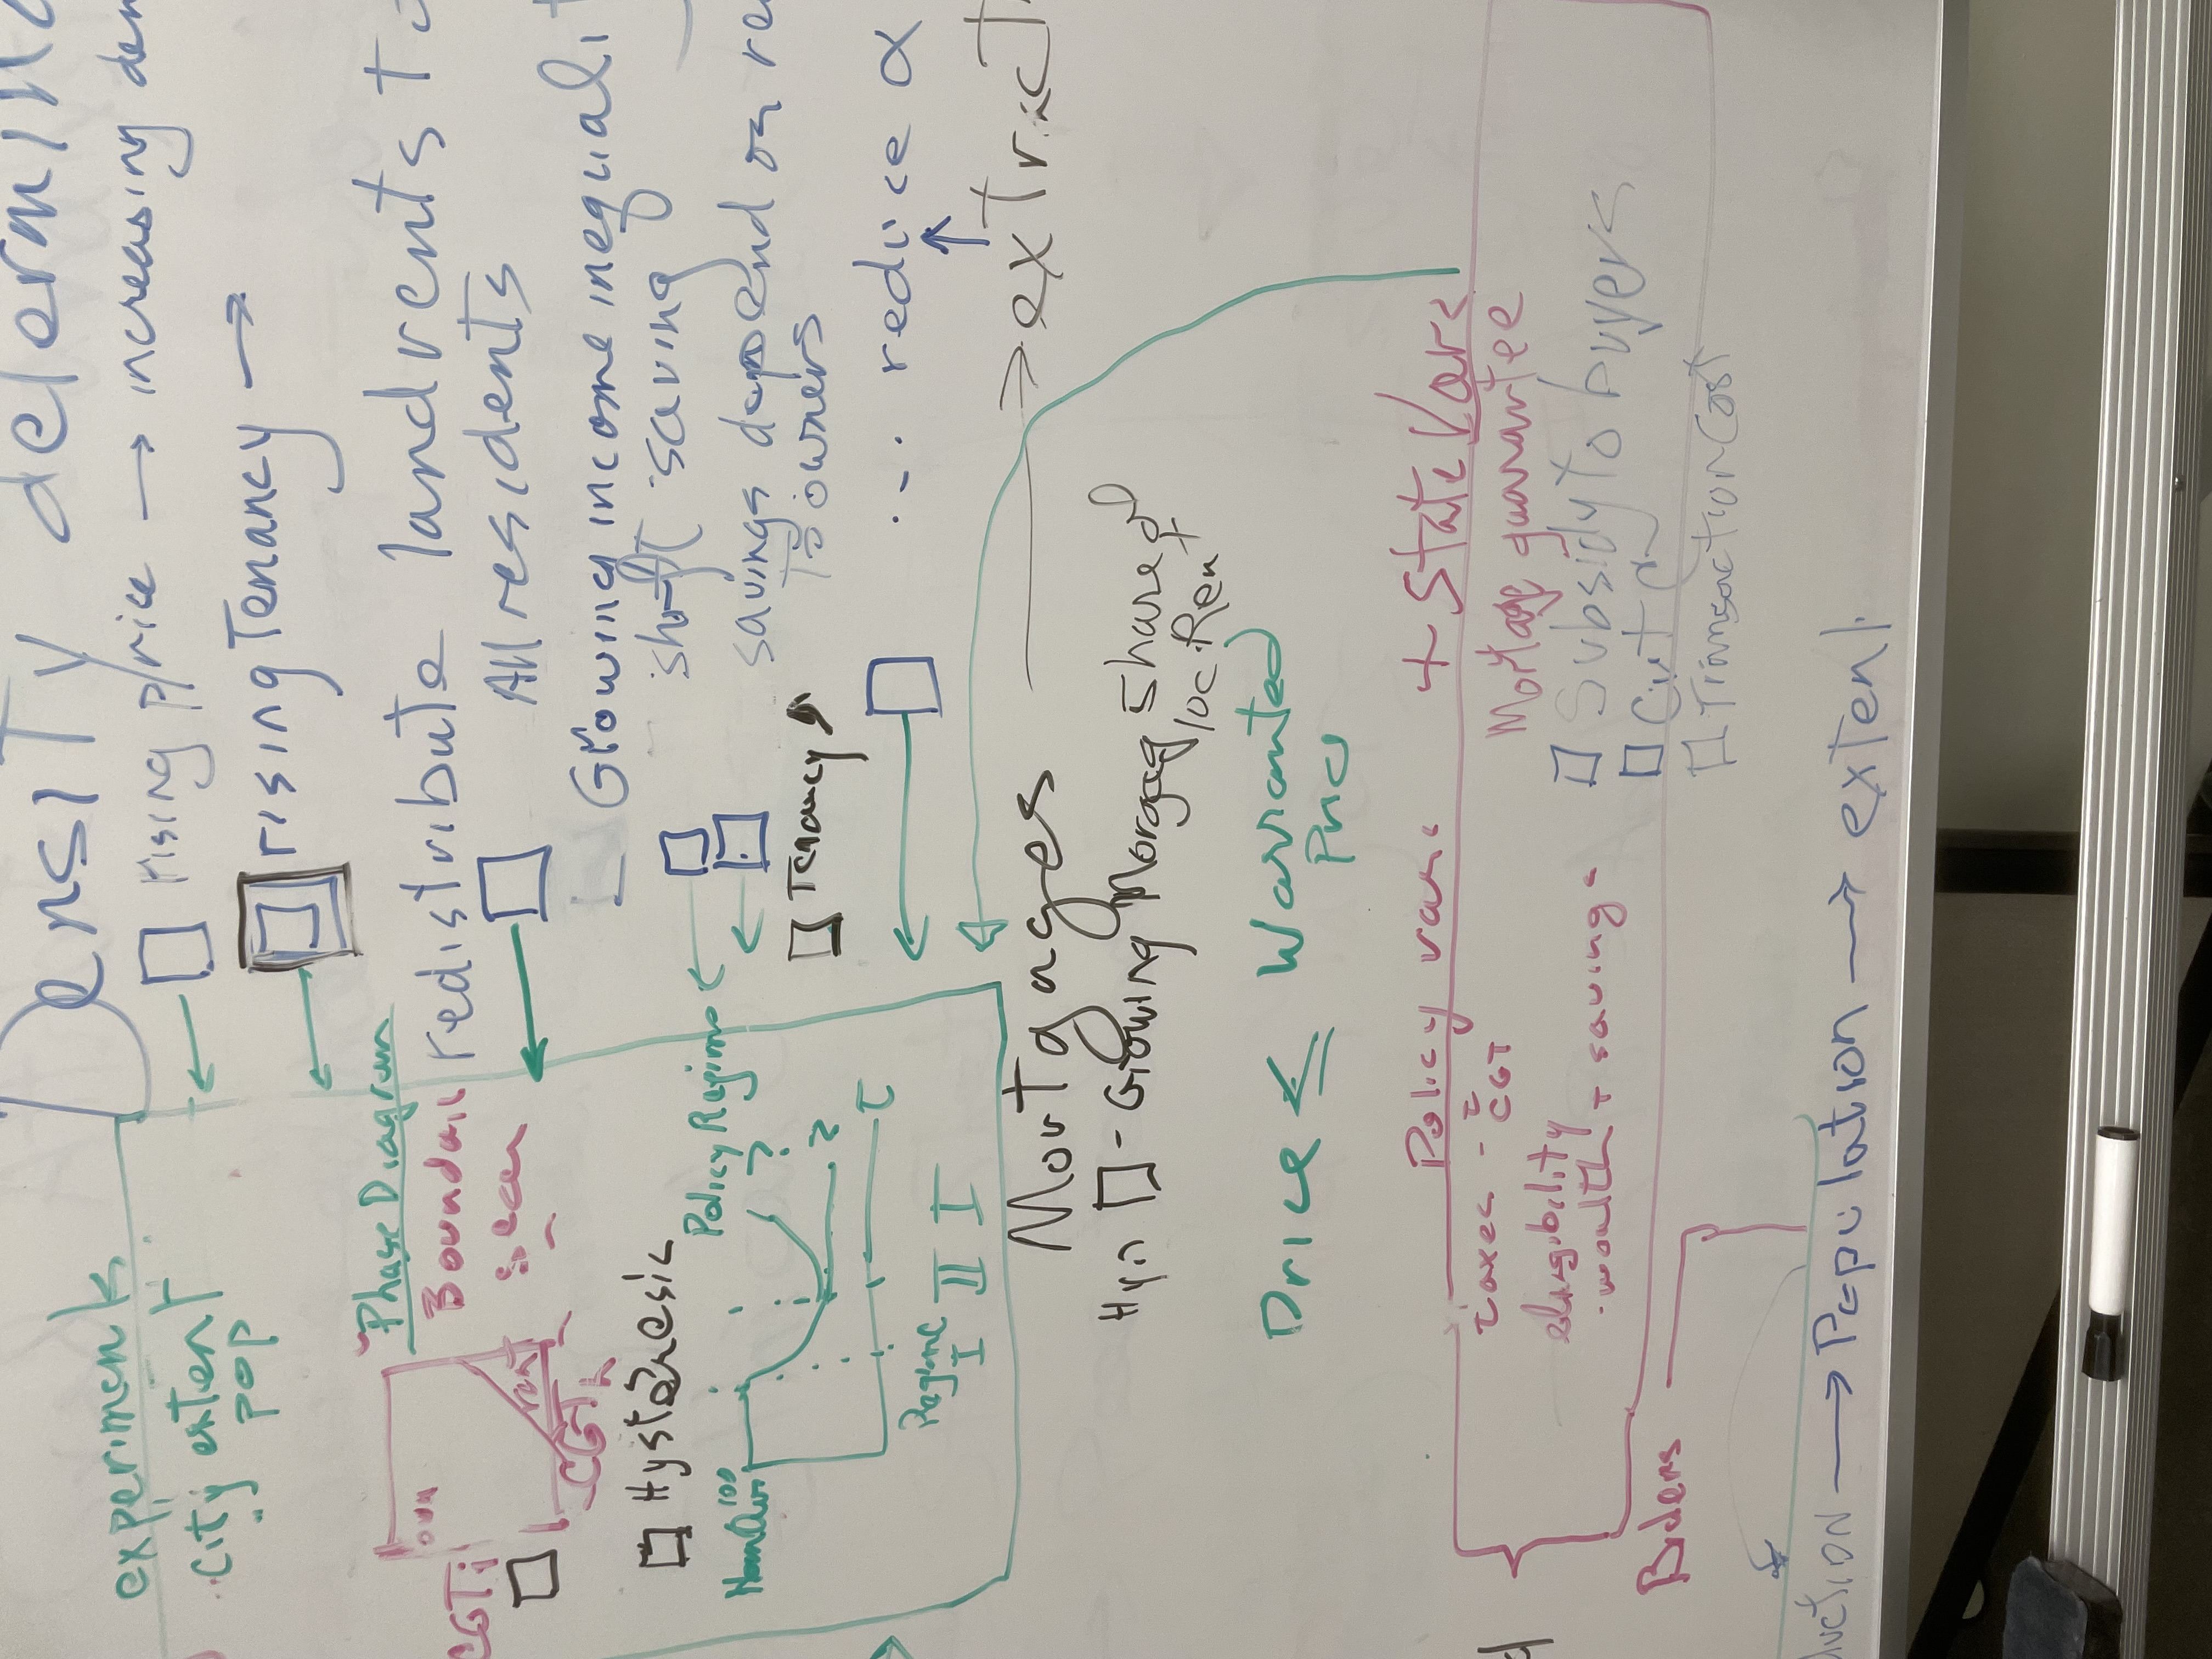
\includegraphics[scale=.5, angle=-90]{IMG_2689.jpg}

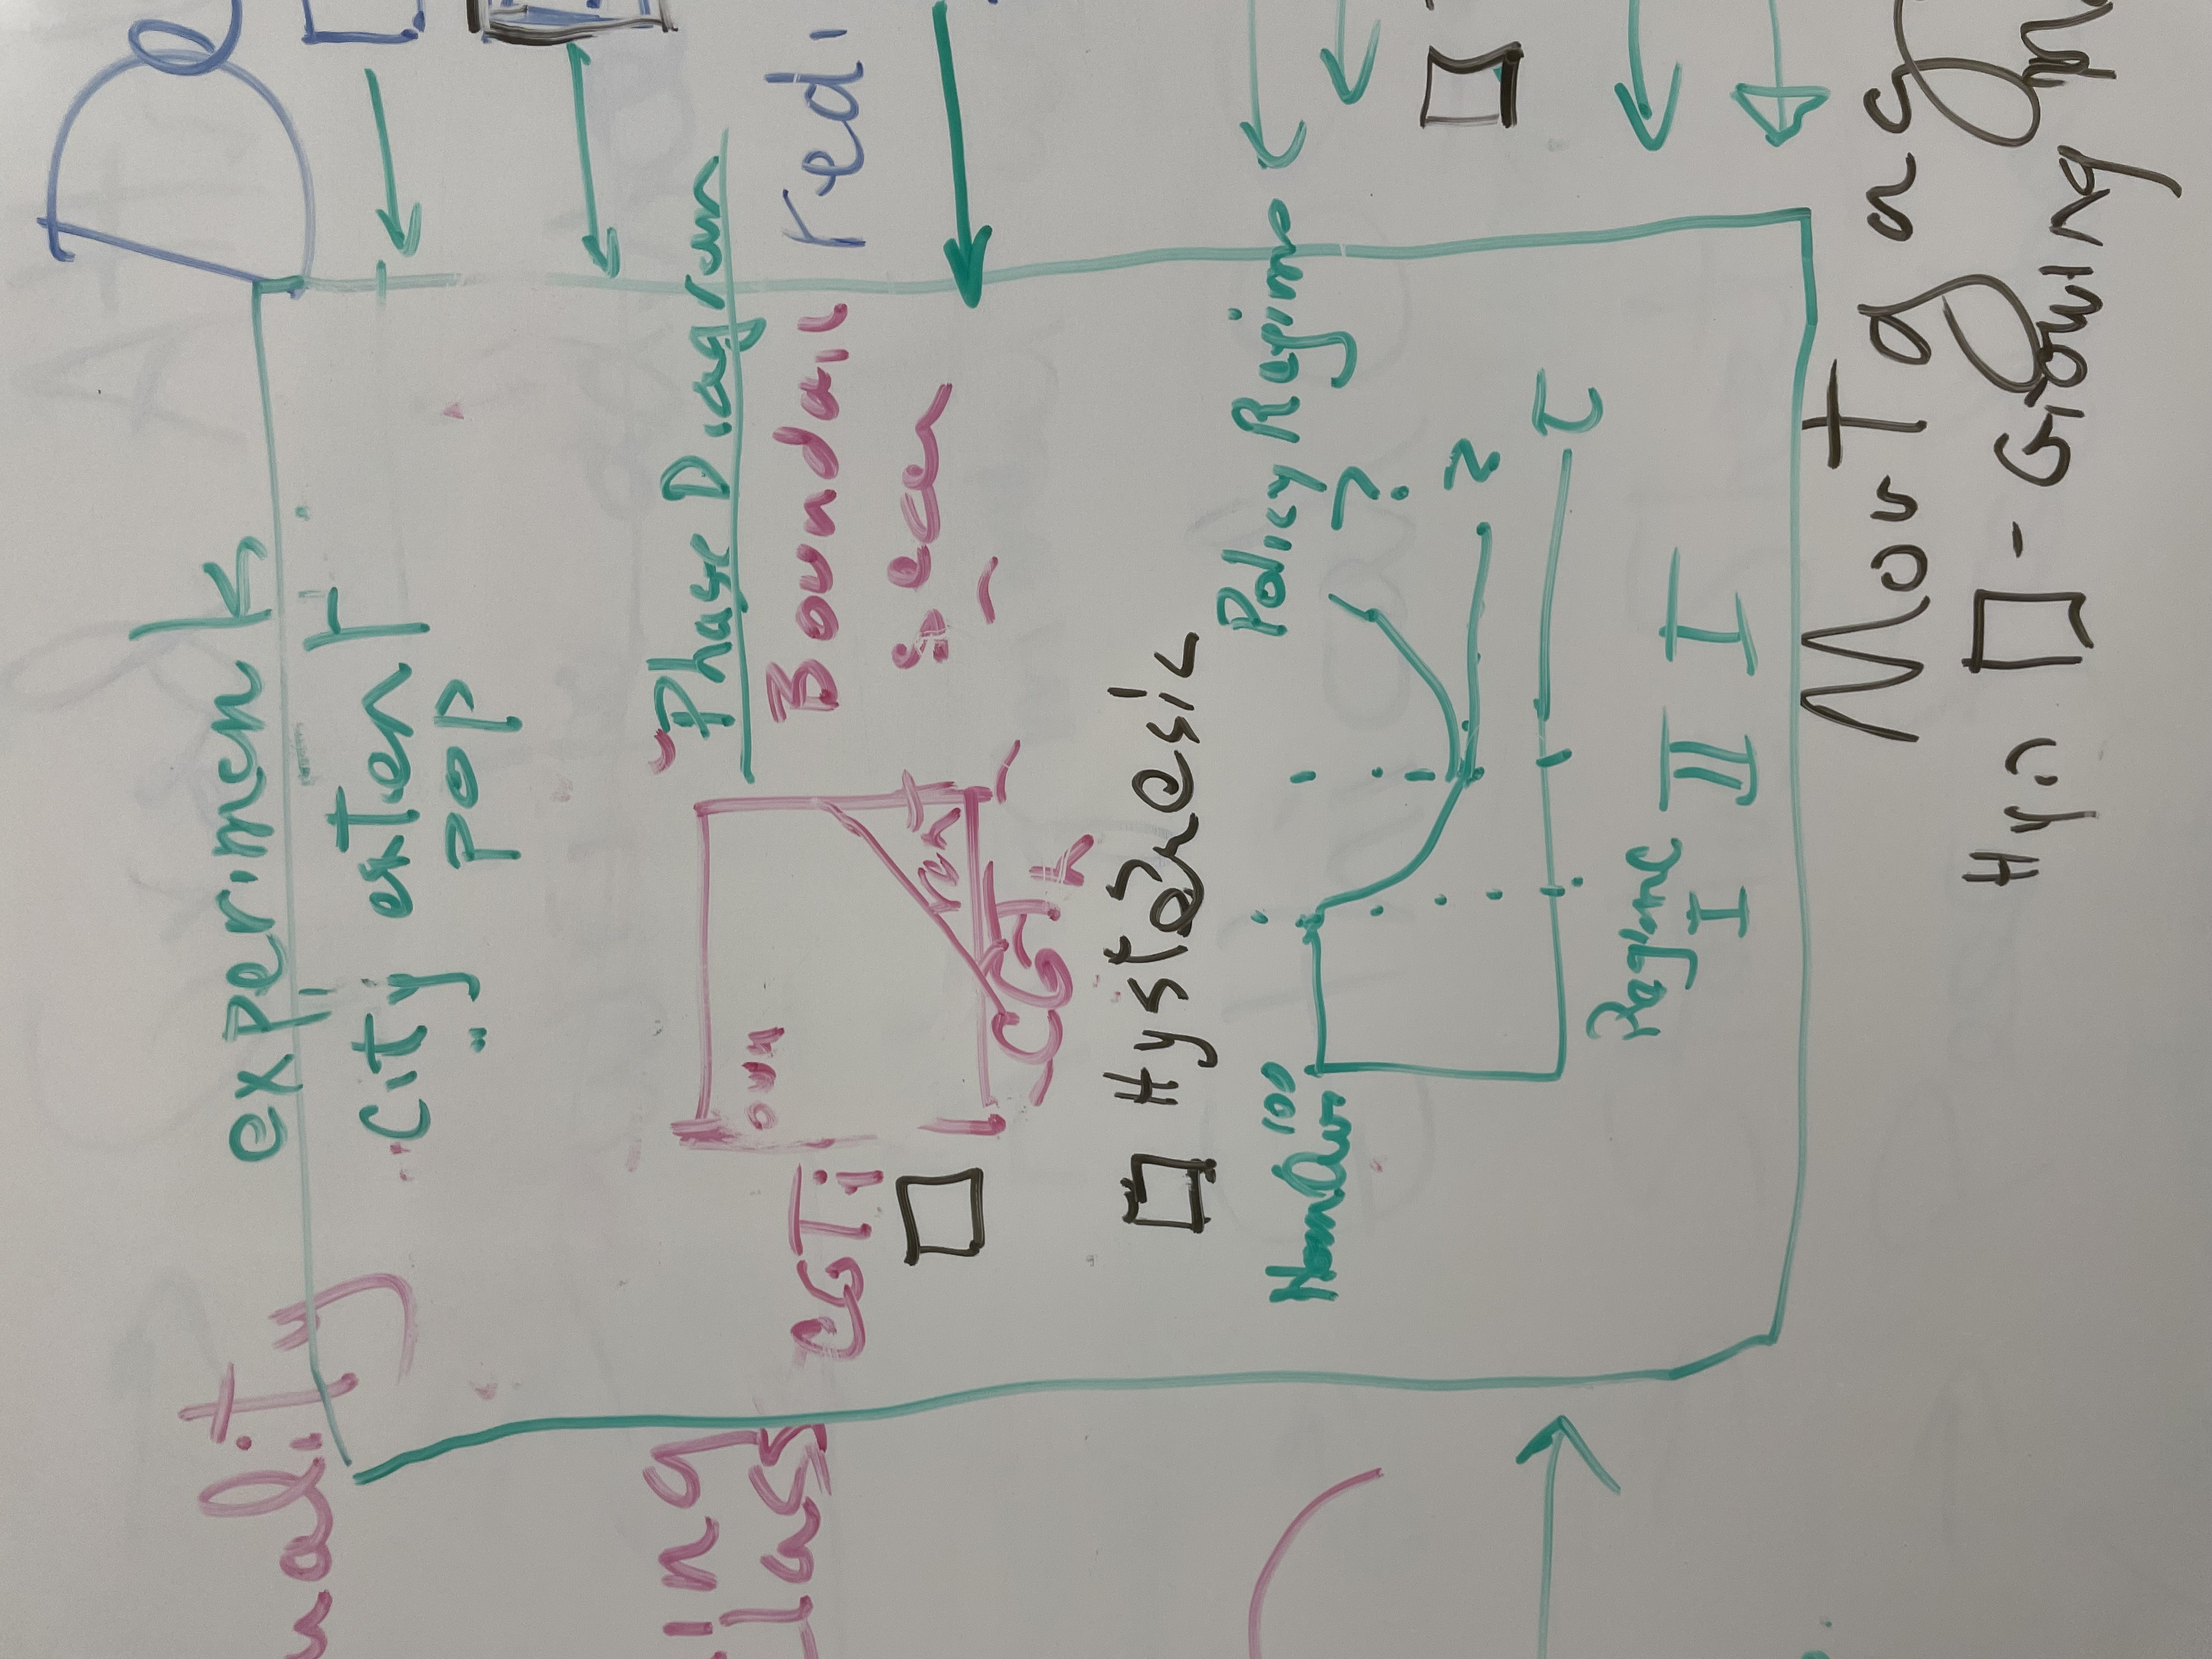
\includegraphics[scale=.5, angle=-90]{IMG_2690.jpg}

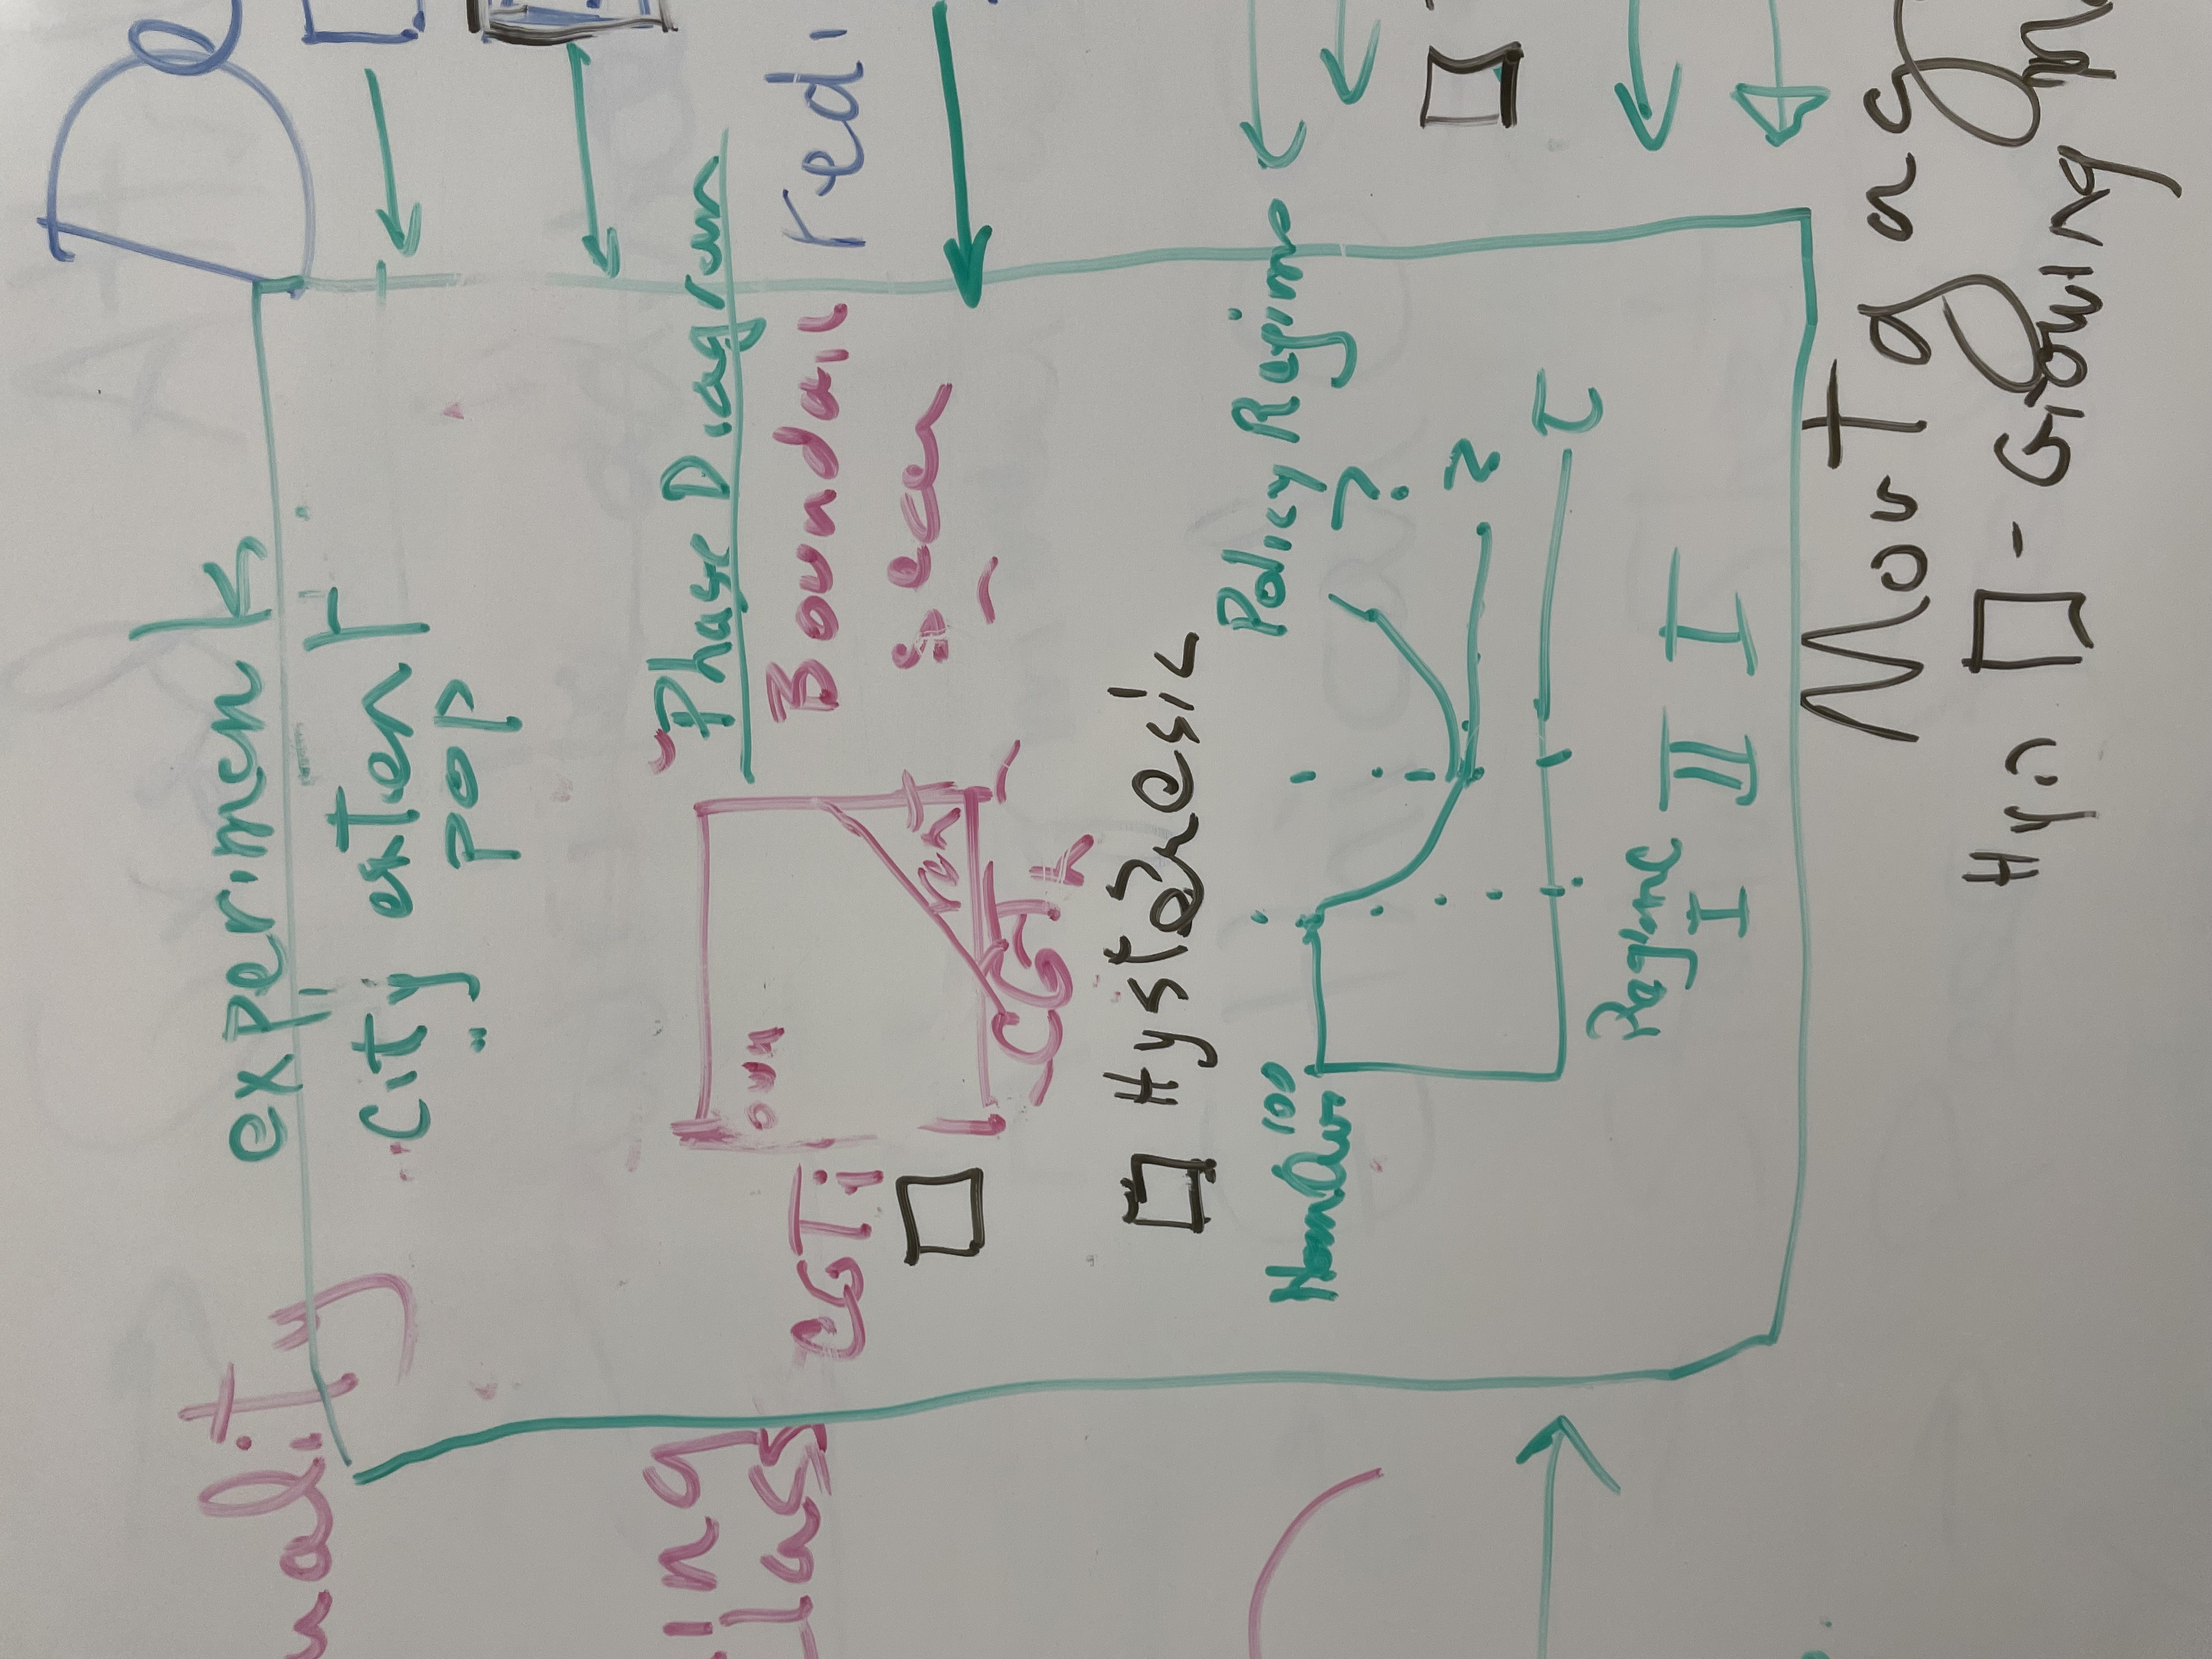
\includegraphics[scale=.5, angle=-90]{IMG_2690.jpg}

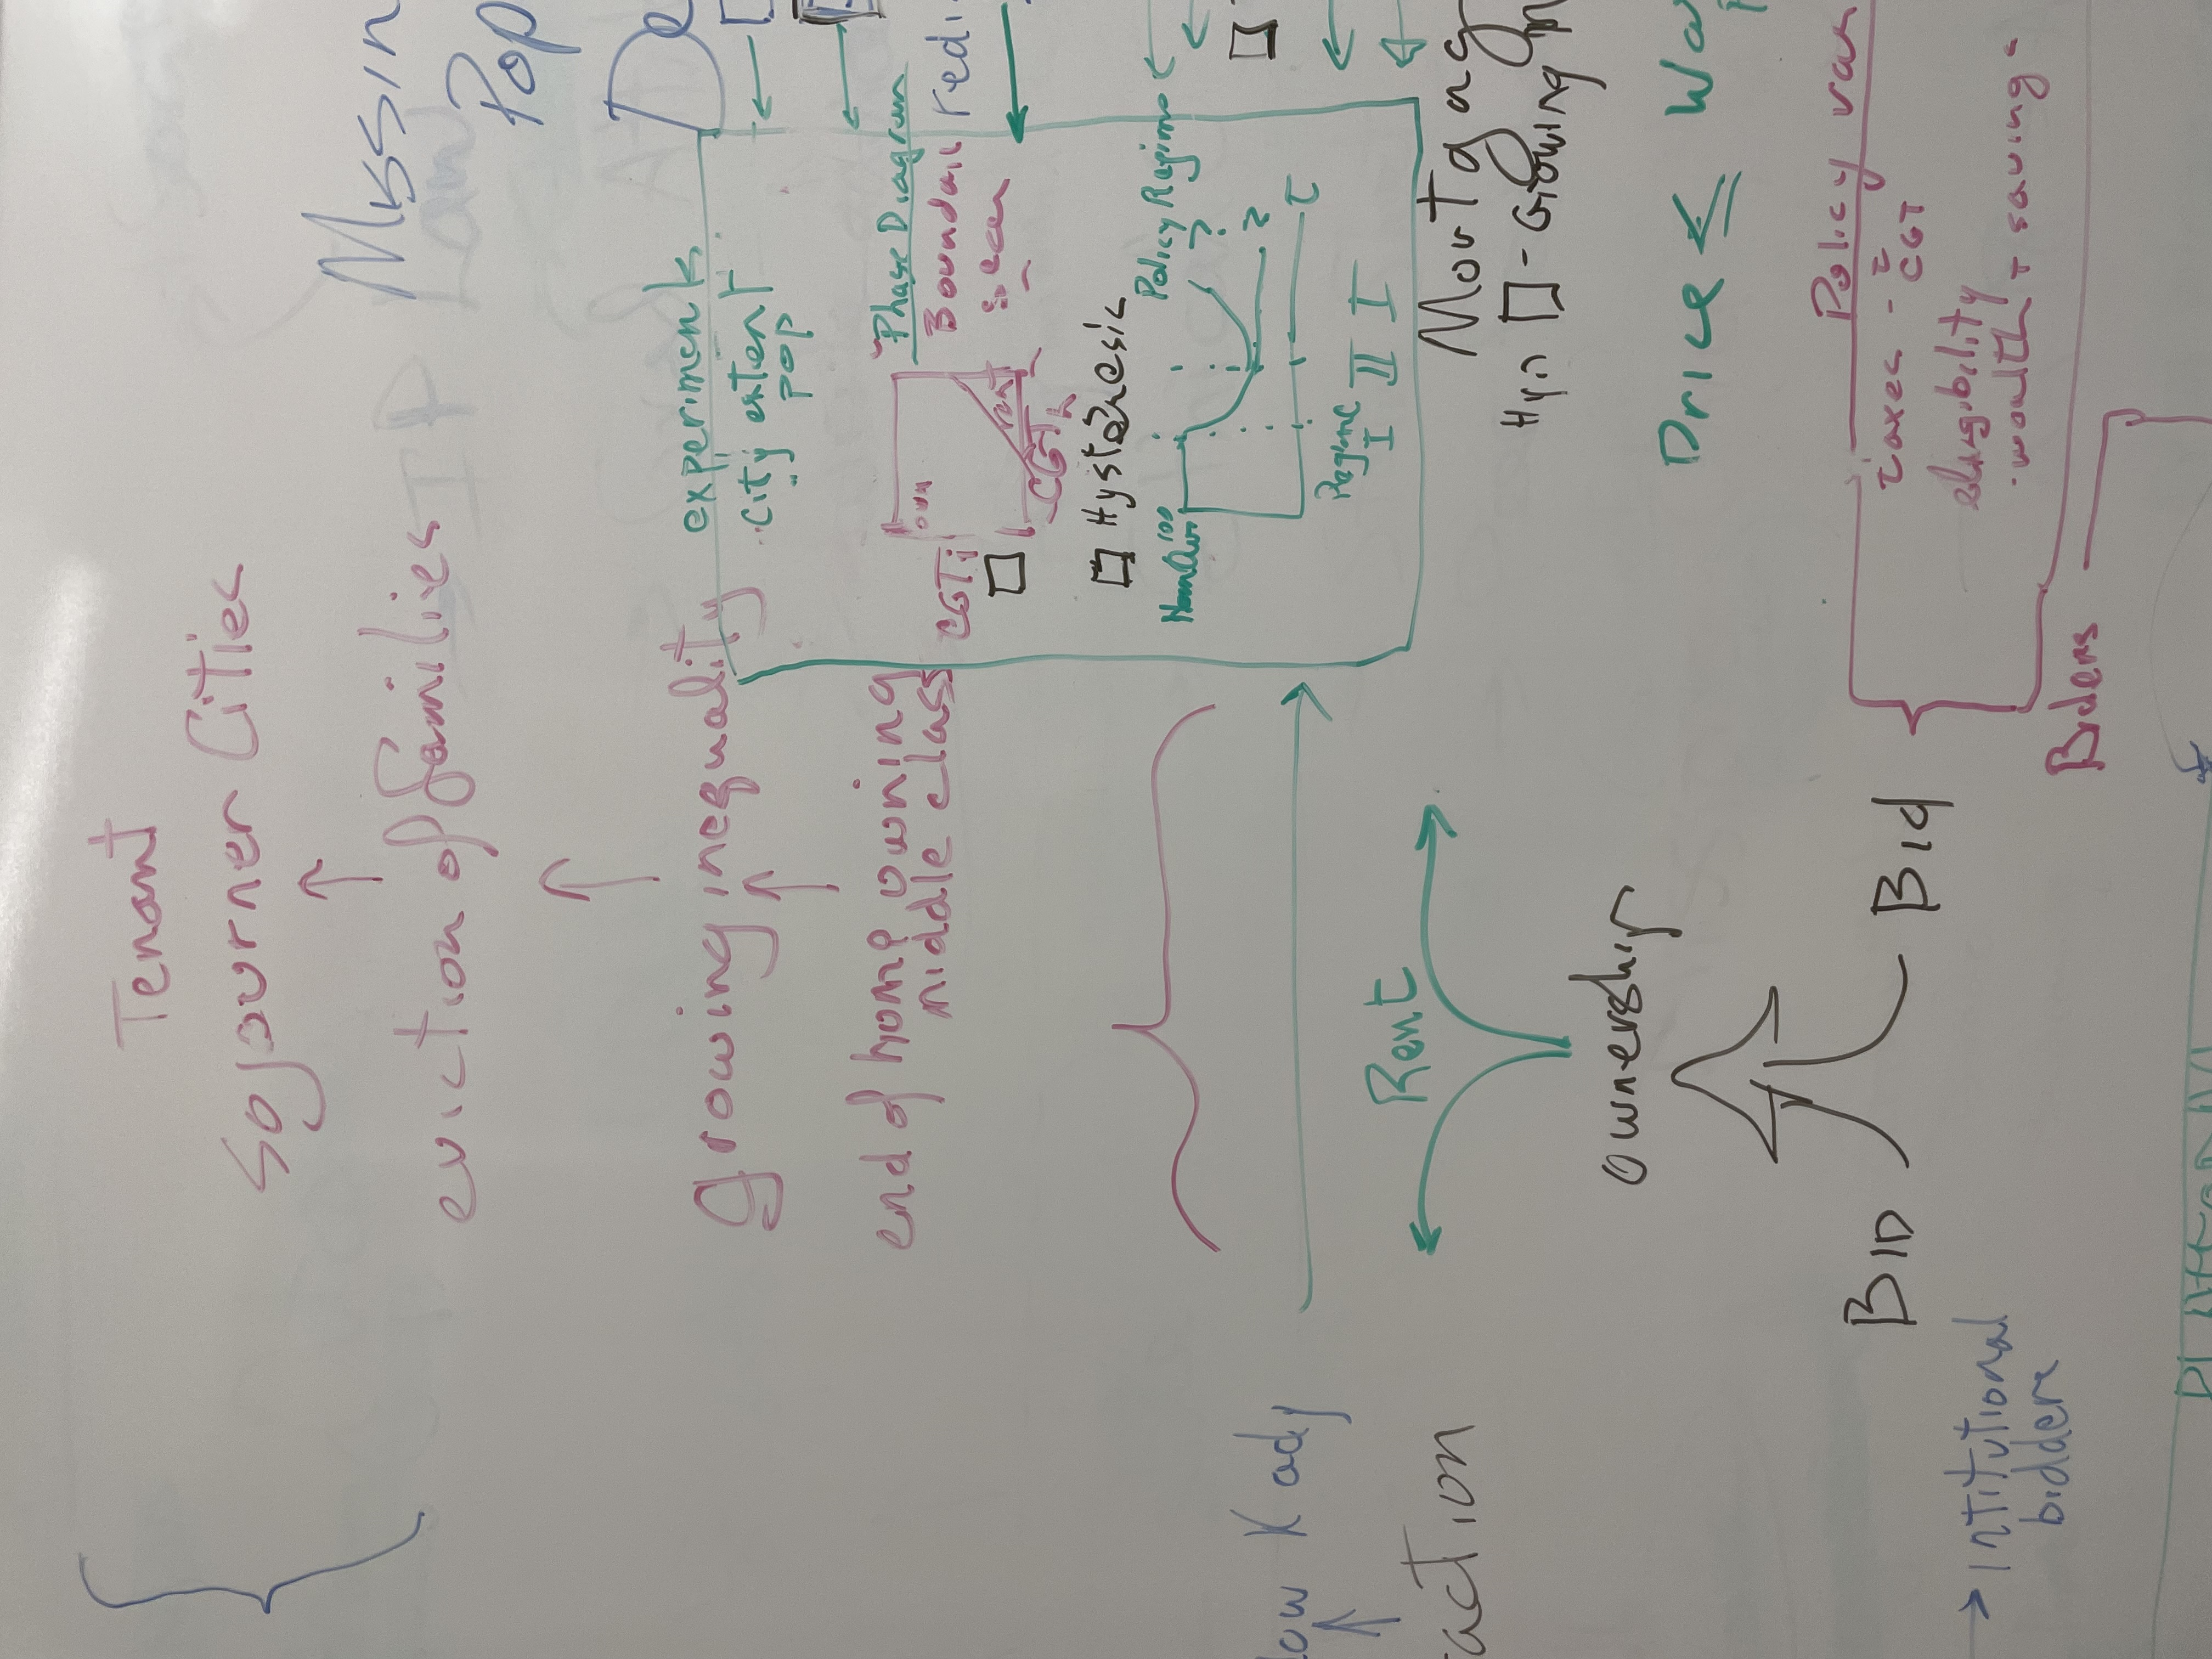
\includegraphics[scale=.5, angle=-90]{IMG_2691.jpg}

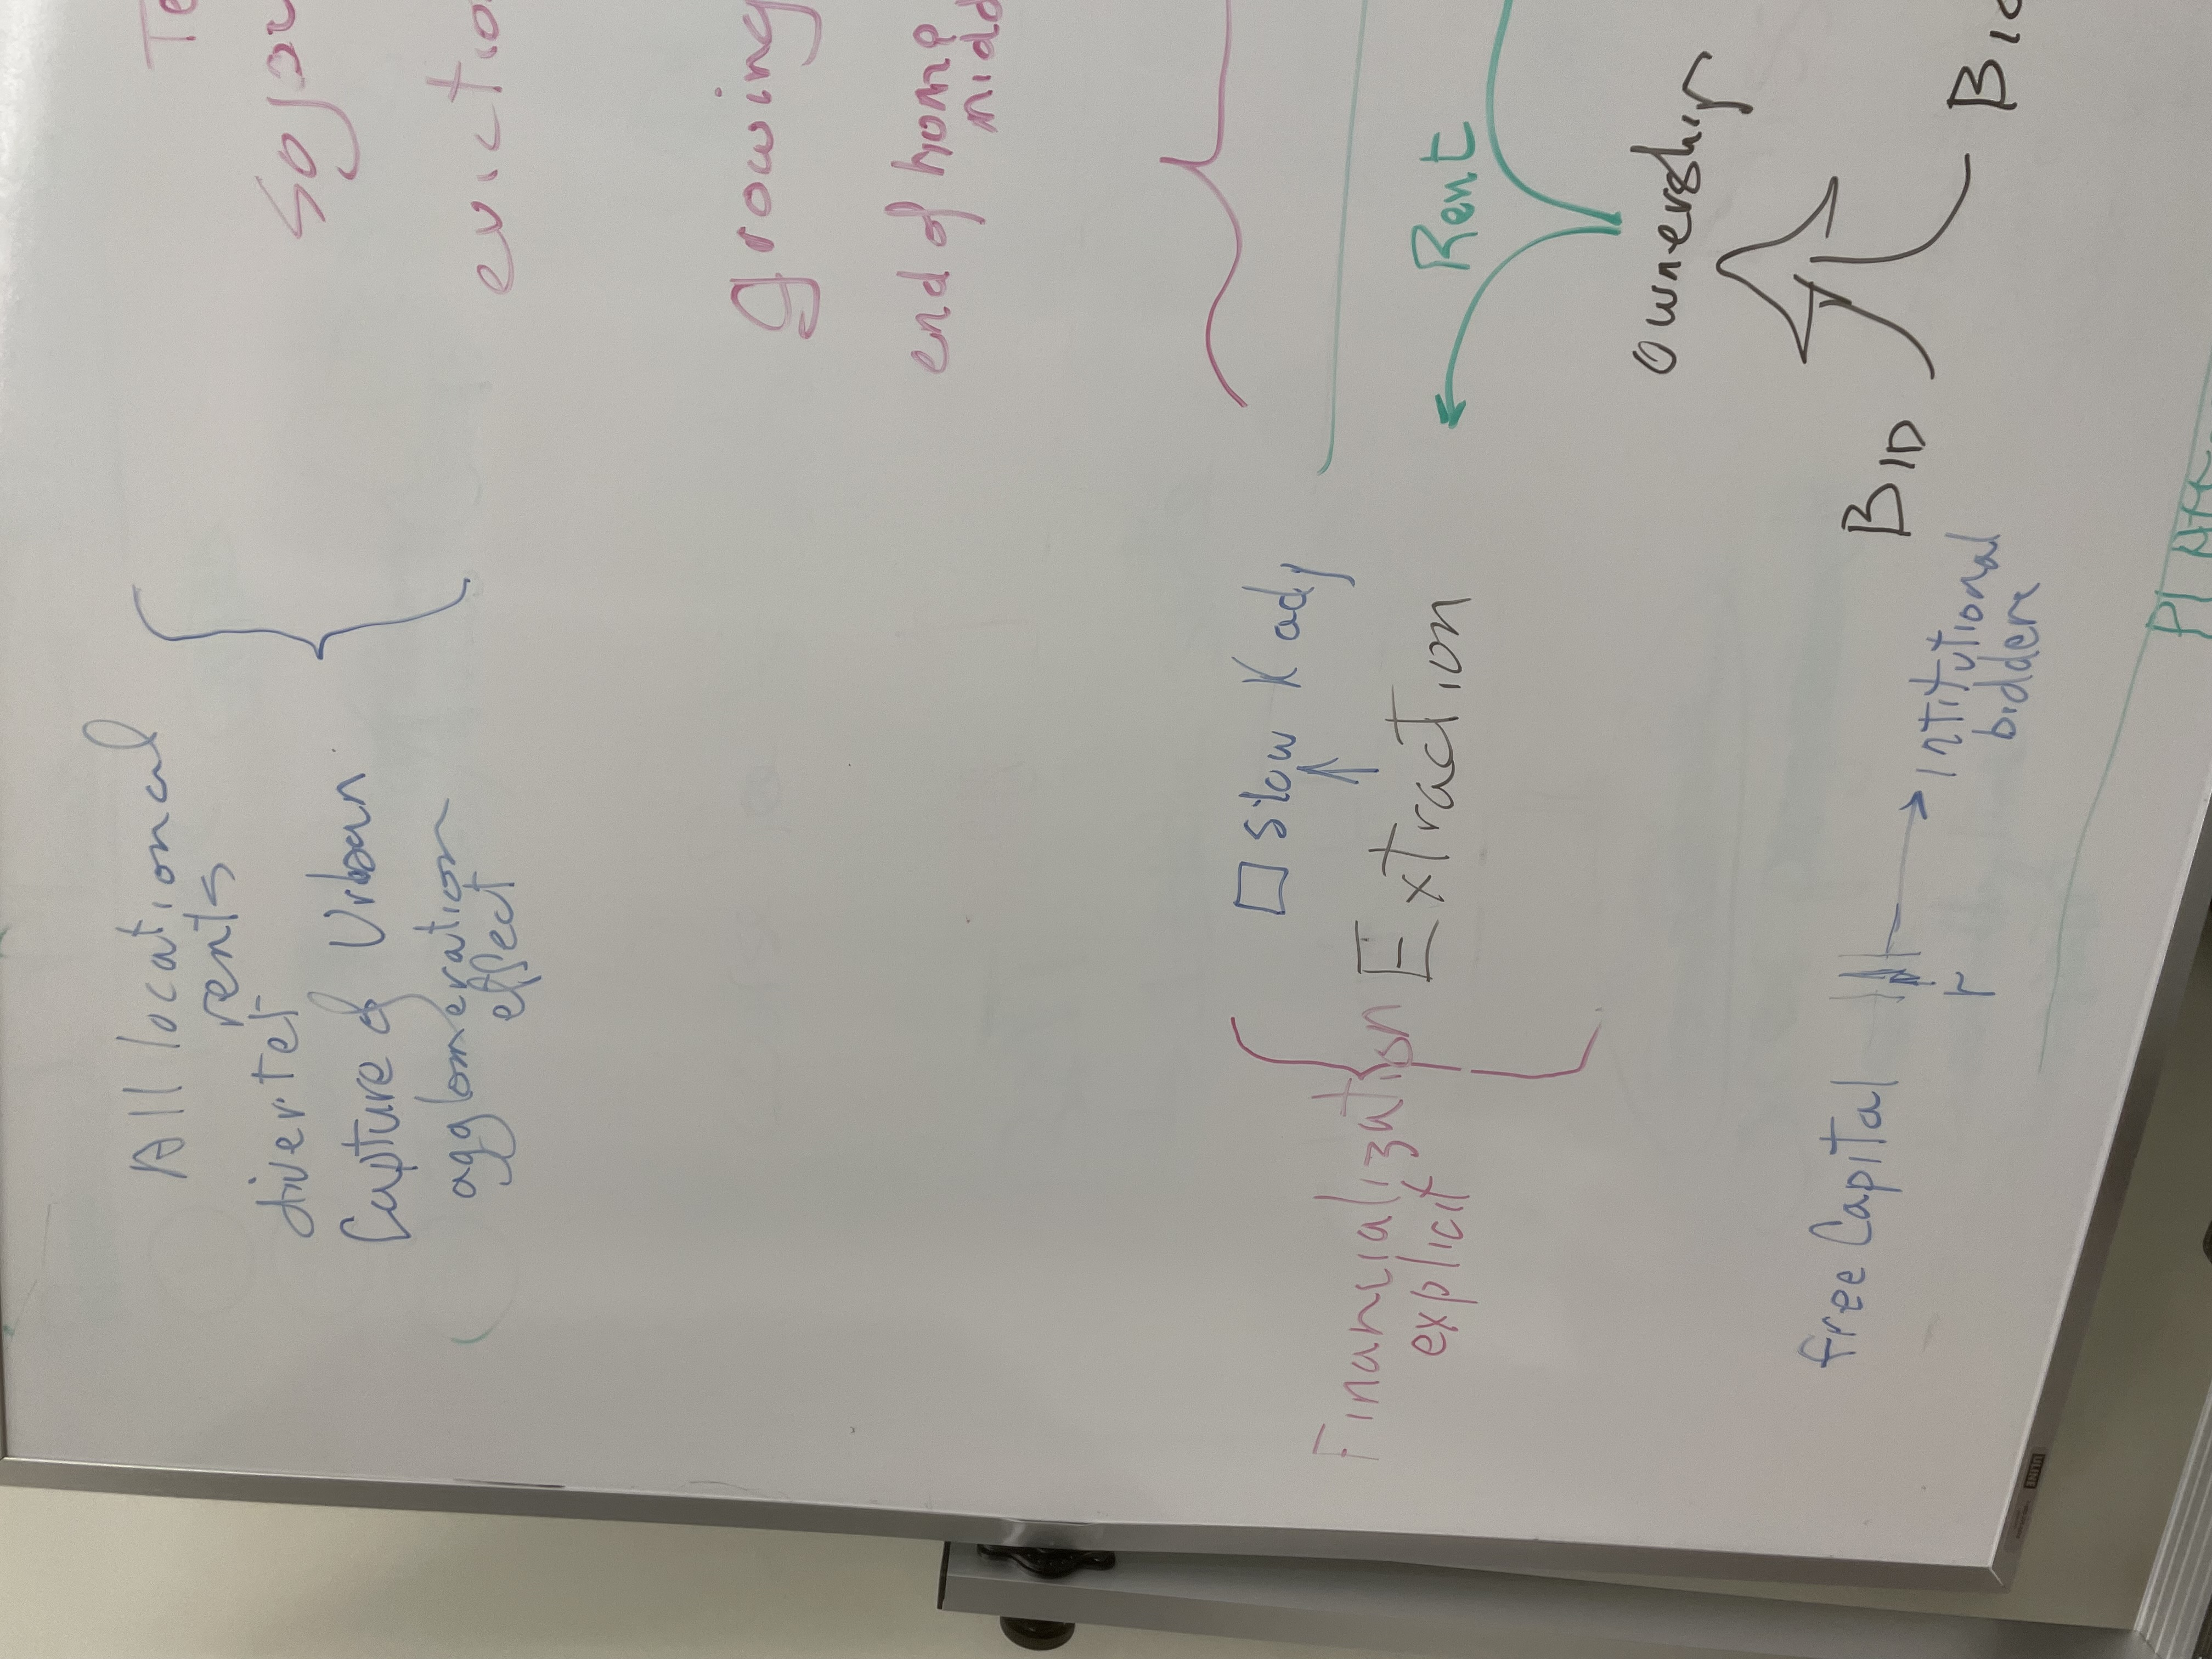
\includegraphics[scale=.5, angle=-90]{IMG_2692.jpg}

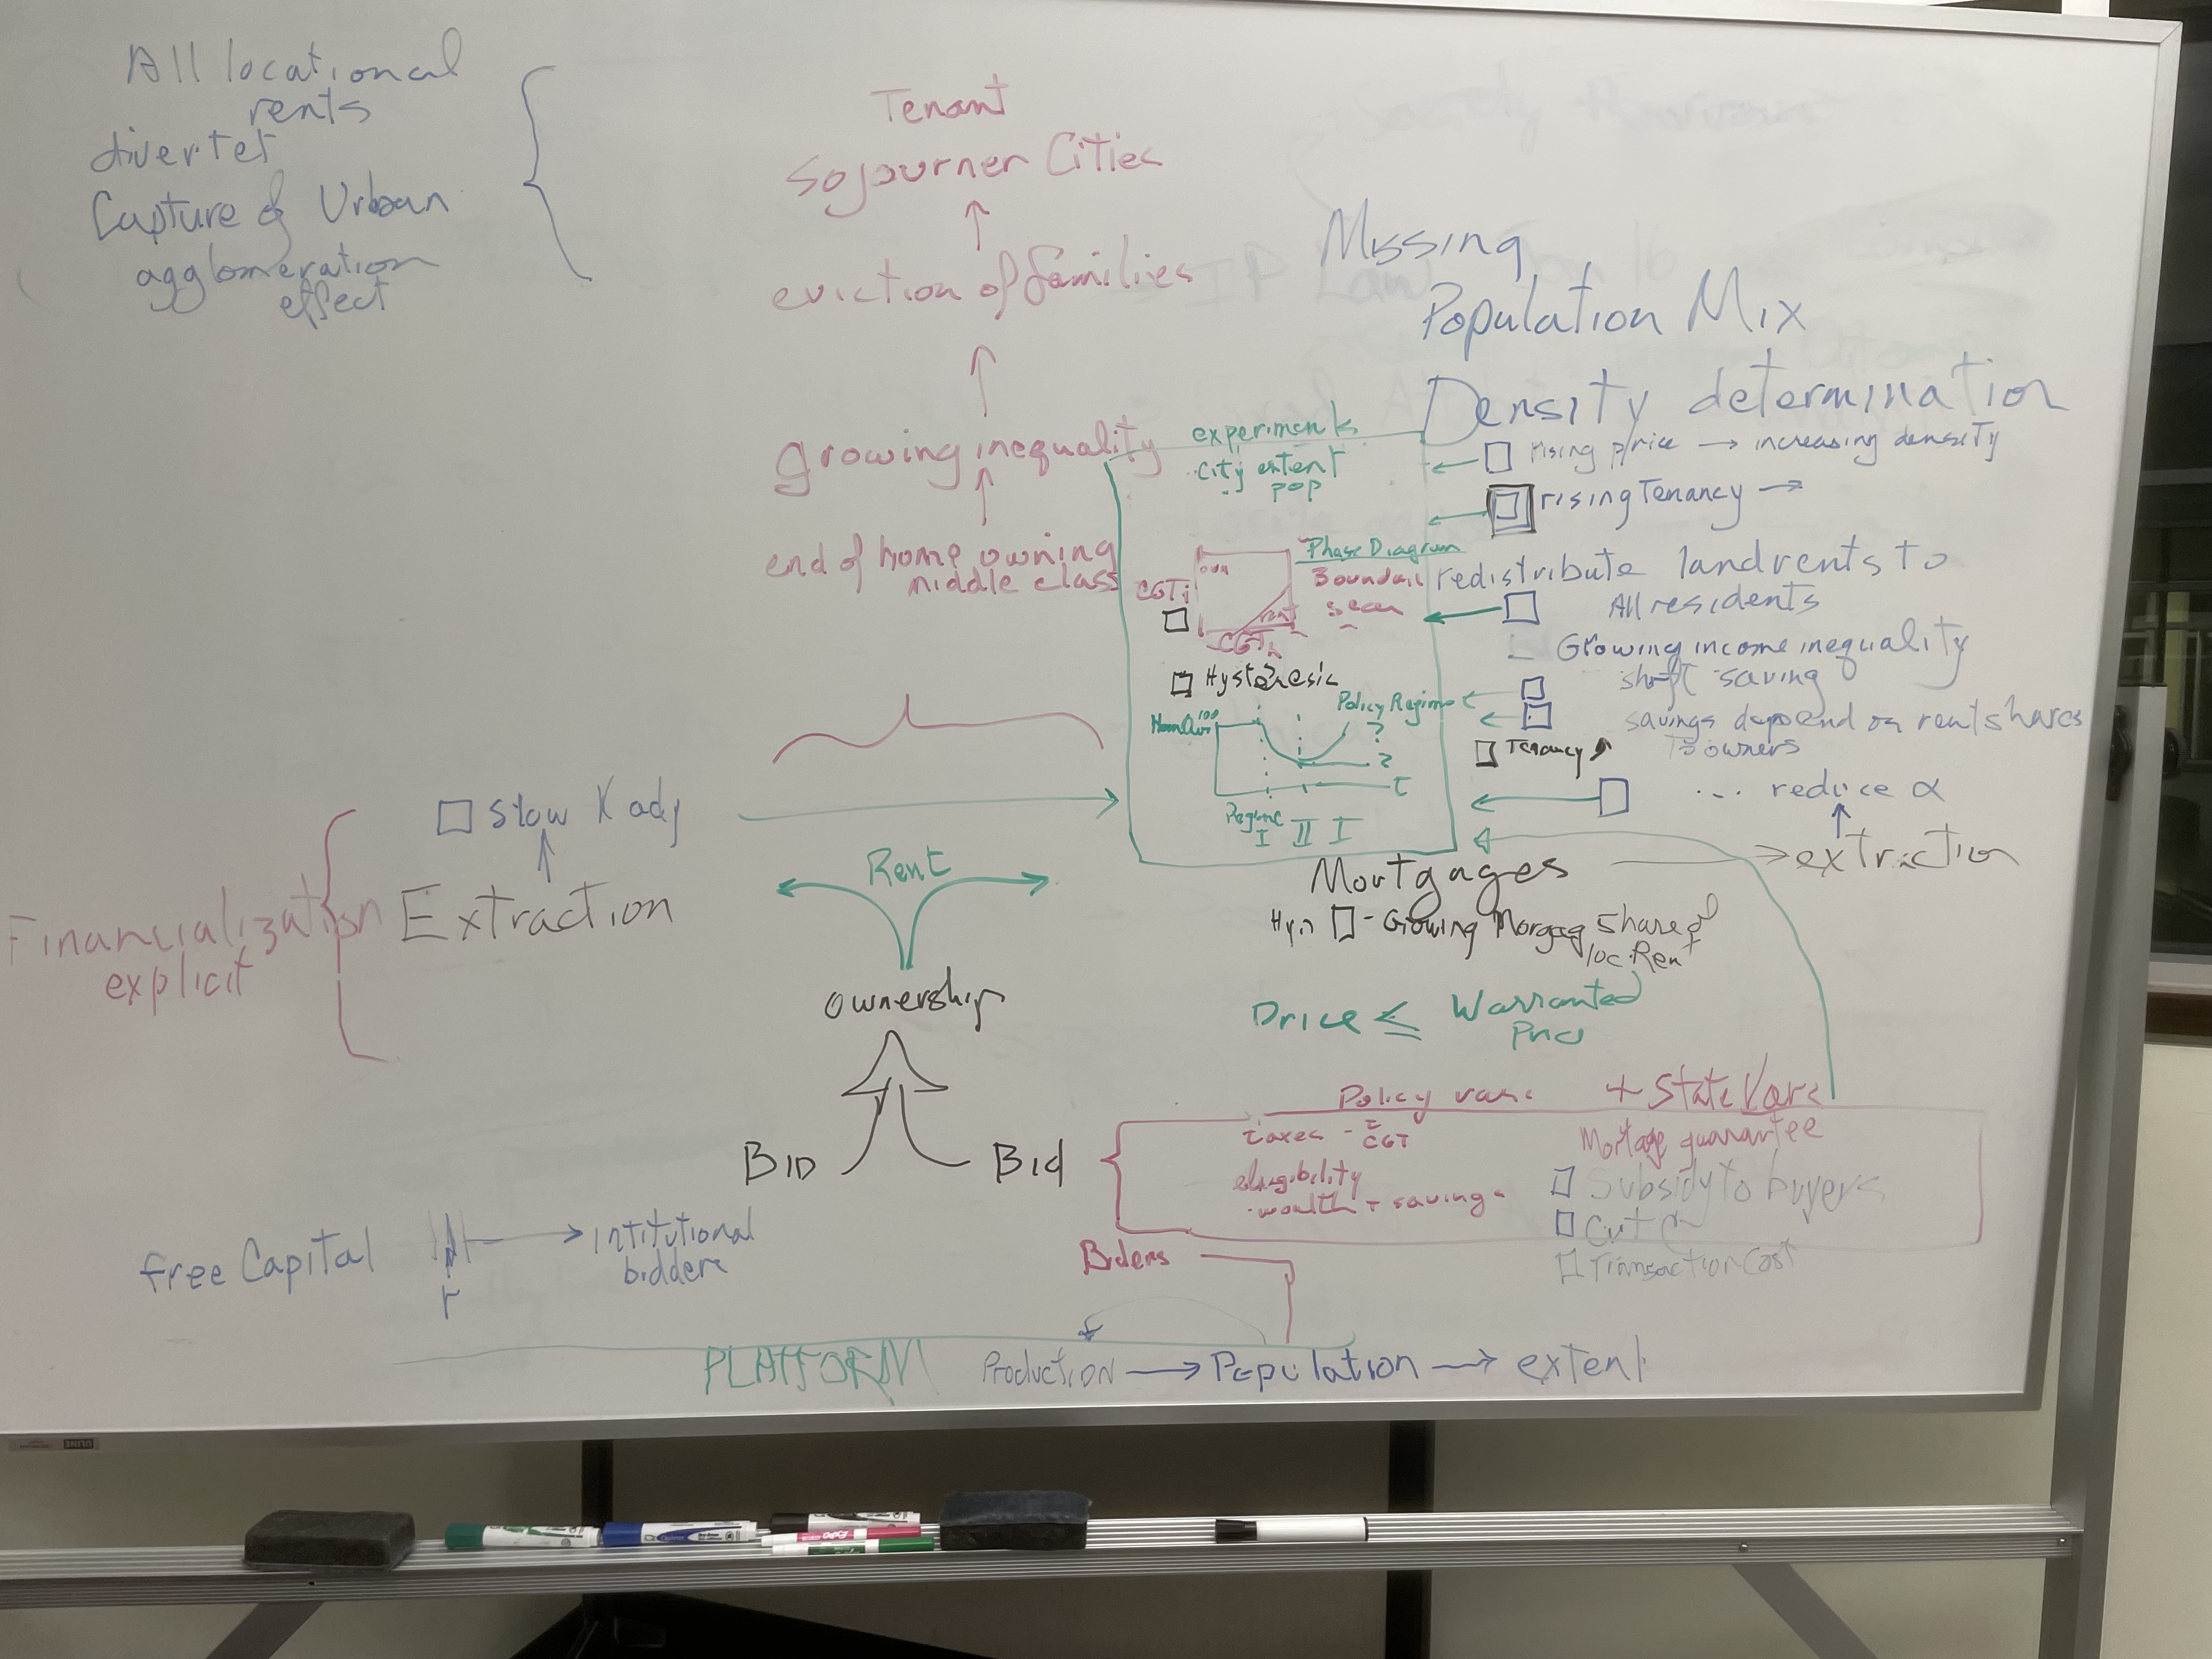
\includegraphics[scale=.5, angle=-90]{IMG_2693.jpg}








\begin{tikzpicture}[scale=.5]
<!-- %\def\bndmax{5}        %https://tex.stackexchange.com/questions/68462/filling-a-complex-region-with-tikz -->
\def\bndmin{0.2}
\def \A {100}
\def \T {1850}
\def \today {2020}
\def \rate {1.05}
\tikzset{func/.style={thick,color=orange!90}}
\end{tikzpicture} 
\end{document} 
 
 